\documentclass[11pt]{article}
\usepackage[utf8]{inputenc}
\usepackage{geometry}
\geometry{a4paper, margin=1in}
\usepackage{hyperref}
\usepackage{graphicx}
\usepackage{tabularx}
\usepackage{booktabs}
\usepackage{enumitem}
\usepackage{tikz}
\usetikzlibrary{shapes,arrows.meta,positioning,fit,backgrounds}

\title{Landslide Identification — Test Results \\ \large Baseline AlexNet + HMM (results0)}
\author{}
\date{2026-03-12}

\begin{document}

\maketitle

\noindent\textbf{GPU:} NVIDIA RTX 2000 Ada Generation \\
\textbf{Environment:} conda landslide-ml (PyTorch cu124, Python 3.10) \\

\section{Motivation: Why AlexNet + HMM as the Baseline?}

This is the first experiment (r0) in the landslide identification pipeline. The architecture choices were driven by the following reasoning:

\begin{enumerate}
    \item \textbf{AlexNet as a starting point:}\\
          AlexNet is one of the simplest and most well-understood deep CNN architectures (5 convolutional layers + 3 fully connected layers). Starting with a lightweight model allows us to establish a \textit{performance floor} --- any subsequent architectural change must demonstrably beat this baseline to justify its added complexity. Additionally, AlexNet's small parameter count ($\sim$62M) and fast training time make it ideal for rapid prototyping on the HR-GLDD dataset (2,190 training images).

    \item \textbf{HMM for temporal risk modeling:}\\
          Satellite image classification alone answers ``is there a landslide here?'' but not ``what type is it, and how likely is it to recur?'' A Hidden Markov Model trained on the NASA Global Landslide Catalog (9,471 events across 141 countries) adds a temporal dimension by learning transition probabilities between landslide regimes. This dual-phase (CNN + HMM) design separates visual detection from probabilistic forecasting, allowing each component to be improved independently.

    \item \textbf{Binary classification to keep it simple:}\\
          Before attempting multi-class landslide type classification, a binary (landslide vs non-landslide) formulation provides a clean signal for measuring detection capability. Precision, recall, and F1-score have direct operational meaning: a missed landslide (false negative) could cost lives, while a false alarm (false positive) wastes resources.
\end{enumerate}

\section{Architecture Flowchart}
\begin{center}
    \resizebox{0.9\textwidth}{!}{
    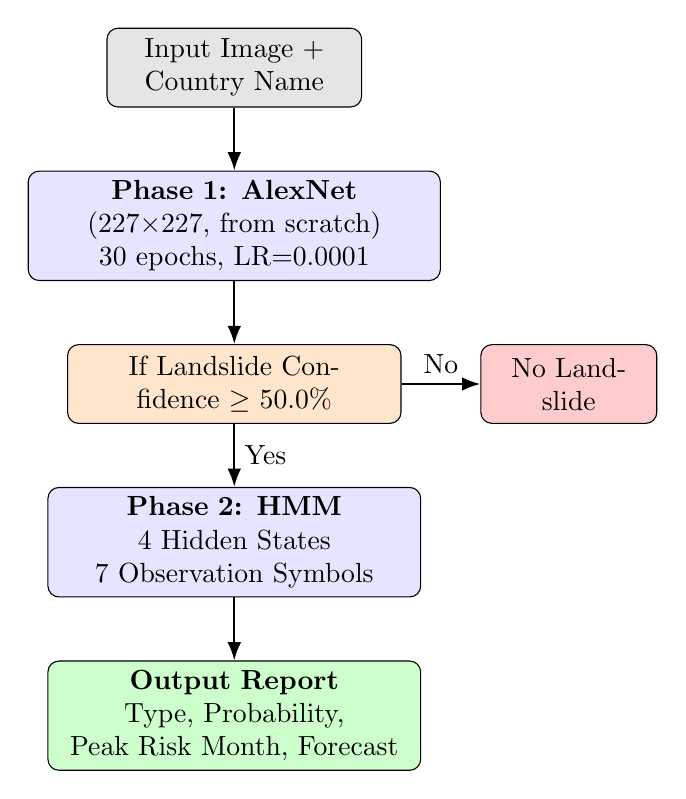
\begin{tikzpicture}[
        node distance=0.8cm and 1cm,
        box/.style={draw, rectangle, rounded corners, align=center, fill=blue!10, text width=3cm, minimum height=1cm},
        arrow/.style={-Latex, thick}
    ]
        % Inputs
        \node[box, fill=gray!20] (input) {Input Image + Country Name};

        % Phase 1
        \node[box, below=of input, text width=5cm] (phase1) {\textbf{Phase 1: AlexNet}\\(227$\times$227, from scratch)\\30 epochs, LR=0.0001};
        \node[box, below=of phase1, fill=orange!20, text width=4cm] (decision) {If Landslide Confidence $\ge$ 50.0\%};

        % Phase 2
        \node[box, below=of decision, text width=4.5cm] (phase2) {\textbf{Phase 2: HMM}\\4 Hidden States\\7 Observation Symbols};

        % Outputs
        \node[box, below=of phase2, fill=green!20, text width=4.5cm] (output) {\textbf{Output Report}\\Type, Probability,\\Peak Risk Month, Forecast};

        % Connections
        \draw[arrow] (input) -- (phase1);
        \draw[arrow] (phase1) -- (decision);
        \draw[arrow] (decision) -- node[right] {Yes} (phase2);
        \draw[arrow] (phase2) -- (output);

        % No branch
        \node[box, right=of decision, fill=red!20, text width=2cm] (no_ls) {No Landslide};
        \draw[arrow] (decision) -- node[above] {No} (no_ls);

    \end{tikzpicture}
    }
\end{center}

\section{Single Image Prediction Test}

\noindent \textbf{Image path:} data/processed/test/landslide/ls\_test\_0008.jpg \\
\textbf{Country:} Nepal \\
\textbf{Forecast:} 3 steps

\vspace{0.3cm}
\noindent \textbf{Phase 1 — AlexNet Classification}
\begin{itemize}[noitemsep]
    \item Result: LANDSLIDE DETECTED
    \item Confidence: 97.3\%
    \item Checkpoint: checkpoints/alexnet\_best.pth (epoch 13, val\_acc=78.55\%)
\end{itemize}

\vspace{0.3cm}
\noindent \textbf{Phase 2 — HMM Type Prediction}
\begin{itemize}[noitemsep]
    \item Landslide type: Landslide
    \item Occurrence probability: 39.6\%
    \item Peak risk month: July
    \item Future forecast (next 3 events):
    \begin{itemize}
        \item Step 1: Landslide (48.0\%)
        \item Step 2: Landslide (64.2\%)
        \item Step 3: Landslide (69.4\%)
    \end{itemize}
\end{itemize}

\noindent \textbf{Final verdict:} LANDSLIDE DETECTED — Type: Landslide (occurrence probability: 39\%)

\section{Phase 1 — Full Test Set Evaluation}

\noindent \textbf{Test set:} 699 images (211 landslide + 488 non\_landslide) \\
\textbf{Device:} CUDA (NVIDIA RTX 2000 Ada Generation)

\vspace{0.3cm}
\begin{table}[h]
    \centering
    \begin{tabular}{@{}ll@{}}
        \toprule
        \textbf{Metric} & \textbf{Value} \\ \midrule
        Accuracy  & 78.54\% \\
        Precision & 62.06\% \\
        Recall    & 74.41\% \\
        F1-Score  & 67.67\% \\
        ROC-AUC   & 85.53\% \\ \bottomrule
    \end{tabular}
    \caption{Phase 1 test set metrics (binary classification).}
\end{table}

\subsection{Confusion Matrix}
\begin{table}[h]
    \centering
    \begin{tabular}{@{}lcc@{}}
        \toprule
        & \textbf{Pred: non\_landslide} & \textbf{Pred: landslide} \\ \midrule
        \textbf{Actual: non\_landslide} & 392 & 96 \\
        \textbf{Actual: landslide}      &  54 & 157 \\ \bottomrule
    \end{tabular}
    \caption{Confusion matrix (binary).}
\end{table}

\subsection{Per-class Breakdown}
\begin{table}[h]
    \centering
    \begin{tabular}{@{}lcccc@{}}
        \toprule
        \textbf{Class} & \textbf{Precision} & \textbf{Recall} & \textbf{F1-Score} & \textbf{Support} \\ \midrule
        non\_landslide & 0.88 & 0.80 & 0.84 & 488 \\
        landslide      & 0.62 & 0.74 & 0.68 & 211 \\
        macro avg      & 0.75 & 0.77 & 0.76 & 699 \\
        weighted avg   & 0.80 & 0.79 & 0.79 & 699 \\ \bottomrule
    \end{tabular}
    \caption{Per-class classification report.}
\end{table}

\noindent\textbf{Plots saved:}
\begin{itemize}[noitemsep]
    \item plots/confusion\_matrix.png
    \item plots/roc\_curve.png
\end{itemize}

\section{Phase 2 — HMM Model Summary}

\begin{itemize}
    \item \textbf{Dataset:} NASA Global Landslide Catalog (nasa\_glc.csv)
    \item \textbf{Records:} 9,471 events | 1988–2016 | 141 countries
    \item \textbf{Sequences:} 112 country-level sequences | 9,442 total observations
\end{itemize}

\noindent\textbf{Hidden states (4):}
\begin{enumerate}[noitemsep, start=0]
    \item Shallow Landslide
    \item Deep Landslide
    \item Debris Flow
    \item Rockfall
\end{enumerate}

\noindent\textbf{Observation symbols (7):}
Complex Landslide (232), Debris Flow (173), Earth Flow (3), Landslide (6756), Mudslide (1818), Rockfall (483), Translational Slide (6)

\vspace{0.3cm}
\noindent\textbf{Training log-likelihood:} $-7314.96$ \\
\textbf{Checkpoint saved:} checkpoints/hmm\_model.pkl \\
\textbf{Encoder saved:} checkpoints/hmm\_encoder.pkl

\section{Training Summary}

\subsection{AlexNet}
\begin{table}[h]
    \centering
    \begin{tabular}{@{}ll@{}}
        \toprule
        \textbf{Parameter} & \textbf{Value} \\ \midrule
        Epochs        & 30 \\
        Batch size    & 64 (GPU) \\
        Learning rate & 0.0001 (StepLR: step=10, gamma=0.1) \\
        Best epoch    & 13 \\
        Best val acc  & 78.55\% \\
        Training plot & plots/training\_history.png \\ \bottomrule
    \end{tabular}
    \caption{AlexNet training configuration.}
\end{table}

\subsection{HMM}
\begin{table}[h]
    \centering
    \begin{tabular}{@{}ll@{}}
        \toprule
        \textbf{Parameter} & \textbf{Value} \\ \midrule
        Hidden states  & 4 \\
        Iterations     & 100 (Baum-Welch) \\
        Log-likelihood & $-7314.96$ \\ \bottomrule
    \end{tabular}
    \caption{HMM training configuration.}
\end{table}

\end{document}
